\section{Introduction}

Modern sequential recommenders such as \base~\cite{kang2018sasrec}
provide a strong backbone for modeling user behavior sequences,
yet real-world catalogs are dominated by cold-start and long-tail
items where collaborative signals are sparse. Item text (titles,
descriptions, reviews) offers semantic cues that can improve
generalization, but it also introduces an operational tension:
lightweight features (e.g., \tfidf) are cheap and surprisingly
strong, while \llm-derived embeddings can be richer yet
substantially more expensive in extraction, storage, and serving.

Two practical observations motivate this work. First, once a
strong \tfidf baseline is in place (e.g., +20.0\% HR@10 and
+38.7\% NDCG@10 on Beauty under full ranking), the marginal
gains from adding \llm features can be small and domain-dependent,
making it unclear when multi-view prompting is worth the extra
cost. Second, model selection in industry often relies on fast
sampled evaluation (uniform-100 negatives), but
sampled metrics can disagree with full-ranking metrics and even
mis-rank models~\cite{krichene2020sampledmetrics}; this mismatch
is particularly harmful when improvements concentrate on
cold-start/long-tail strata.

\model addresses this contradiction with a simple
``prepare--interact--align'' recipe (Figure~\ref{fig:cover}):

\textbf{(1) Prepare} (representation level): We normalize
and whiten each text view independently to address three failure
modes---scale mismatch across views, view-to-view correlation,
and cross-view redundancy. Whitening decorrelates multi-view
channels, making subsequent interactions more learnable.

\textbf{(2) Interact} (fusion level): We use an explicit cross
network (DCN-V2) to learn high-order ID$\times$text feature
crosses. While Transformer self-attention models sequence-level
item--item dependencies, it does not explicitly capture
feature-level interactions between ID embeddings and text
embeddings; DCN-V2 fills this gap through element-wise products
gated by learned weight matrices.

\textbf{(3) Align} (objective level): We align each text view
to the collaborative ID embedding space via InfoNCE contrastive
loss. Alignment targets are (text view $\to$ ID space); positive
pairs are (item's text view, item's ID embedding); negatives are
in-batch items. Cold-start reweighting prevents frequent items
from dominating the alignment signal, ensuring that
low-popularity items receive sufficient gradient updates.

Our contributions are threefold.
\begin{itemize}[leftmargin=*,itemsep=1pt]
  \item We propose \model, a deployable plug-in framework for
    \base that supports a frugal \tfidf-only configuration as
    well as stronger multi-view \llm features under a fixed
    embedding budget.
  \item We benchmark on two Amazon domains (Beauty and
    Toys\&Games) with \textbf{full-ranking} evaluation and
    popularity-stratified metrics, and provide systematic
    ablations (whitening, SE-style gating, cross) alongside robustness
    analyses (hyperparameter sensitivity/stability) in the
    appendix.
  \item We go beyond reporting gains by explaining a key
    phenomenon: whitening and explicit cross can improve
    ranking quality (MRR/NDCG) while slightly hurting recall
    (HR), revealing an HR--ranking trade-off that guides when
    to choose lightweight versus stronger configurations.
\end{itemize}
The rest of the paper is organized as follows: we review
related work, introduce \model and the two-phase training
protocol, present full-ranking results and ablations, and
conclude with analyses and takeaways.

\begin{figure*}[t]
\centering
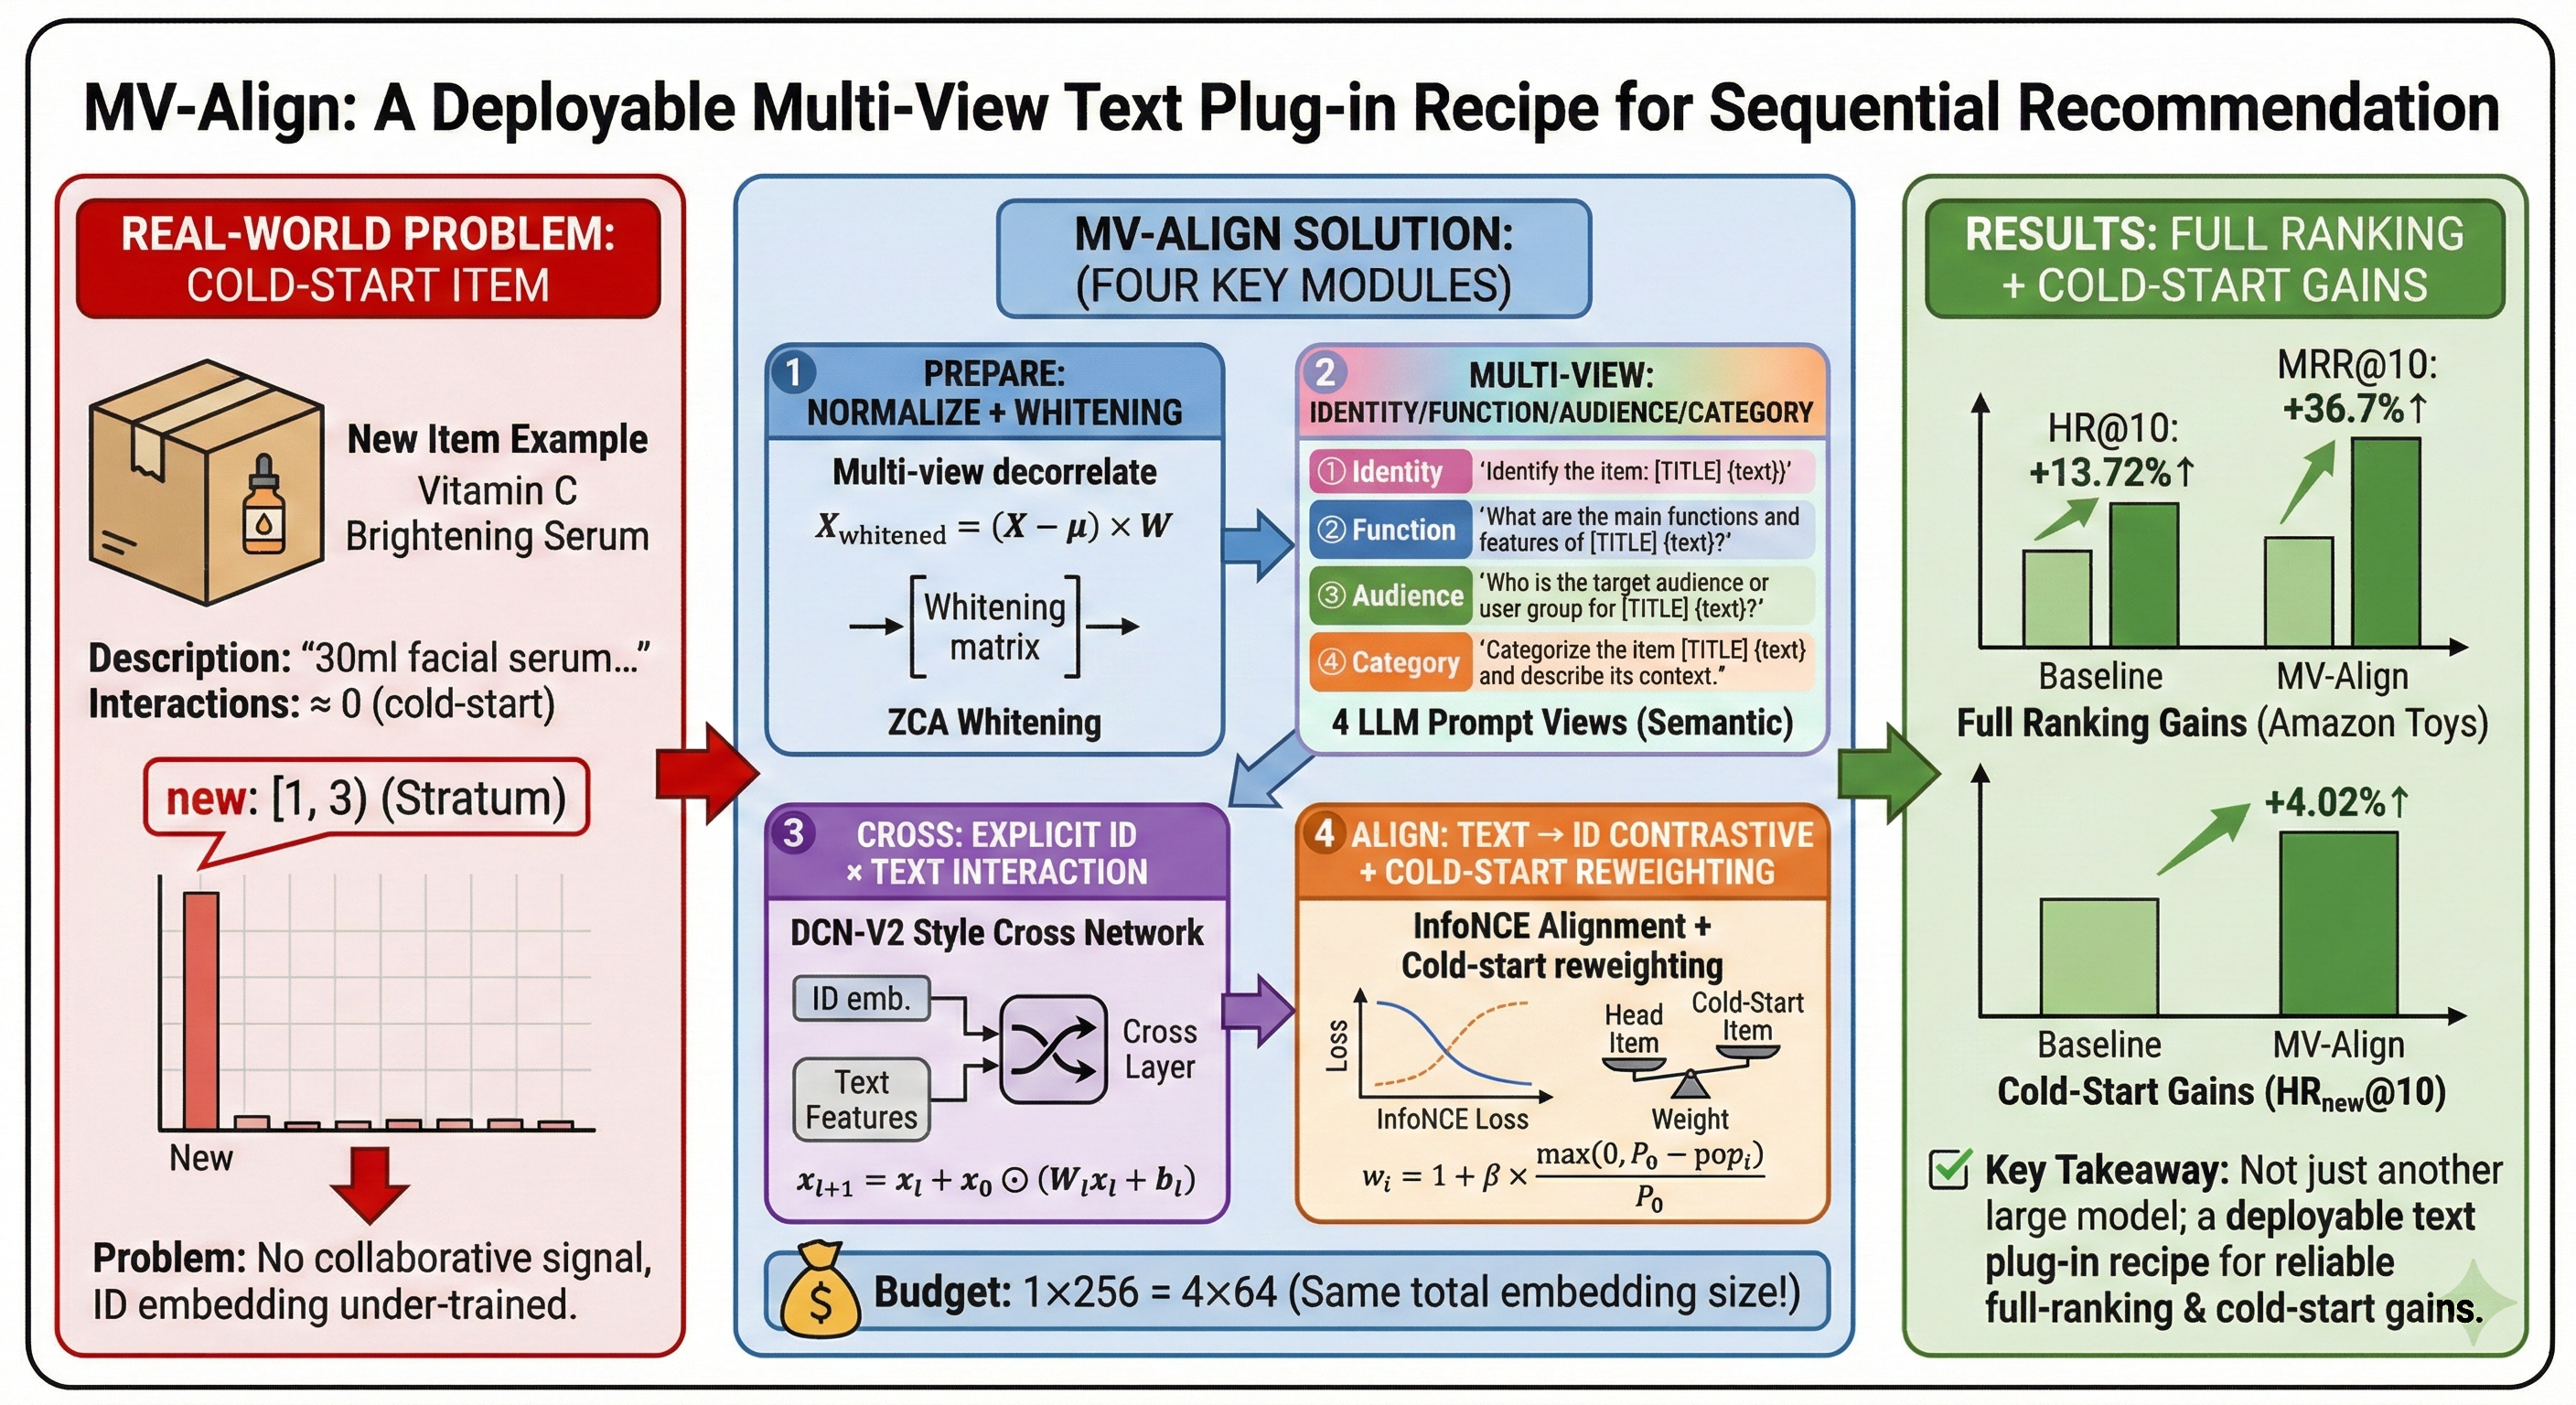
\includegraphics[width=0.95\textwidth]{figures/mv-cover.png}
\caption{Overview of \model: a deployable text plug-in for sequential recommendation.
\textbf{Left}: Cold-start items lack collaborative signals (new stratum: [1,3) interactions).
\textbf{Middle}: Four-module recipe---\textit{Prepare} (normalize+whiten), \textit{Multi-view} (4 LLM prompts), \textit{Cross} (DCN-V2 ID$\times$Text), and \textit{Align} (InfoNCE with cold-start reweighting).
\textbf{Right}: Full-ranking gains (+13.72\% HR@10, +36.7\% MRR@10) and cold-start improvements (+4.02\% HR\_new@10).
Budget: 1$\times$256-d = 4$\times$64-d (same total).}
\label{fig:cover}
\end{figure*}
